\documentclass[12pt]{src/thesis} 
% *****************************************************
% Generate standard “lorem ipsum” text
% *****************************************************
\usepackage{lipsum}
% *****************************************************
% Line numbers for  examiner
% *****************************************************
%\usepackage{lineno}
%\linenumbers
% *****************************************************
% Bibliography
% *****************************************************
\addbibresource{bibliography.bib}
\addbibresource[label=ownpubs]{publications.bib}
% *****************************************************
% Document settings
% *****************************************************
\title{TMD's are little shits and are not to be trusted} %your thesis title,
\author{Cedric Diggory}             %your name
\degree{Doctor of Philosophy in  Defence Against the Dark Arts}    %the degree
\supervisor{Prof. Albus Dumbledore}  %Supervisor name
\college{Department of Mysteries}  %your college
\university{Trinity College Dublin} %your university
\degreedate{\today}         %the degree date
% *****************************************************
% start the document
% *****************************************************
\begin{document}
%this baselineskip gives sufficient line spacing for an examiner to easily
%markup the thesis with comments
\baselineskip=18pt plus1pt
%set the number of sectioning levels that get number and appear in the contents
\setcounter{secnumdepth}{3}
\setcounter{tocdepth}{3}

\maketitle                  % create a title page from the preamble info
%*******************************************************
% Declaration
%*******************************************************
\begin{originality}
I declare that this thesis has not been submitted as an exercise for a degree at this or any other university and it is entirely my own work. 

I agree to deposit this thesis in the University’s open access institutional repository or allow the library to do so on my behalf, subject to Irish Copyright Legislation and Trinity College Library conditions of use and acknowledgement. 
\end{originality}


        % include a dedication.tex file
\include{src/dedication}        % include a dedication.tex file
%*******************************************************
% Acknowledgements
%*******************************************************
\begin{acknowledgements}
\lipsum[1-2]


Thank you all!

\end{acknowledgements}   % include an acknowledgements.tex file
%*******************************************************
% Publications
%*******************************************************

\begin{center}
\vspace*{1.5cm}
{\Large \bfseries Publications}
\end{center}
\vspace{0.5cm}

\begin{refsection}[ownpubs]
    % \small
    \nocite{*} % is local to to the enclosing refsection
    \printbibliography[heading=none]
\end{refsection}		% include an publications.tex file
\begin{abstract}
\lipsum[1-2]

\end{abstract}          % include the abstract
\begin{romanpages}          % start roman page numbering
\thispagestyle{empty}
\tableofcontents            % generate and include a table of contents
\cleardoublepage
\phantomsection
\addcontentsline{toc}{chapter}{\listfigurename}\listoffigures              % generate and include a list of figures
\cleardoublepage
\phantomsection
\addcontentsline{toc}{chapter}{\listtablename}\listoftables
\cleardoublepage
\phantomsection
\addcontentsline{toc}{chapter}{List of Acronyms}
\chapter*{List of Acronyms}
\begin{acronym}[SLCC]
	\acro{LPE}{Liquid Phase Exfoliation}
	\acro{AFM}{Atomic Force Microscopy}
	\acro{SC}{Cholate Hydrate}
\end{acronym}
\newpage
\end{romanpages}            % end roman page numbering
%now include the files of latex for each of the chapters etc
\doublespacing
\chapter{Chapter 1}
%*******************************************************
\section{Introduction}
\lipsum[1]
%*******************************************************
\section{section11}\label{section11}
Chemical equations: \ce{WS2}


Acronyms: \acs{LPE}


Citation\cite{T8} and citation\cite{batteriesSusantyoko2015} in  section \autoref{section11}

Figure: (\autoref{fig:ch03f1})


Table: \autoref{tab:ch04t1}


Equation: \autoref{eq:ch02eq2}


\lipsum[1-4]
%*******************************************************
\section{section12}\label{section12}
\lipsum[1-2]
\begin{table}[ht]
\centering
  \scalebox{0.8}{
  \begin{tabular}{|c|ccccc|}
  \hline
  No.	& Energy 	& 0.1 mJ 	& 0.75 mJ 	& 1.5 mJ 	& 3.0 mJ \\
  		& N 		& cm/GW 	& cm/GW 	& cm/GW 	& cm/GW \\
  \hline
  1 & 7.1 & -33.88 	& 2.95 	& 3.05 	& 3.47	\\
  2 & 5.3 & -24.87 & 3.09 & 0.68 & 1.59 	\\ 
  3 & 5.2 & -15.80 & -1.47 & 0.25 & 0.71 	\\ 
  4 & 4.0 & -13.23 & -1.95 & -0.55 & 0.17 	\\ 
  5 & 3.4 & -11.31 & -4.26 & -1.56 & -0.39 	\\ 
  6 & 2.8 & -8.26 & -4.48 & -1.95 & -0.47 	\\ 
  7 & 2.2 & -7.07 & -4.45 & -2.13 & -0.68 	\\
  \hline
  \end{tabular}
  }
  \caption{
  Size dependent $\beta$\textsubscript{eff}.
  }
  \label{tab:ch04t1}
\end{table}
\lipsum[1-2]
%*******************************************************

\subsection{subsection121 \texorpdfstring{\ce{DS2}}{DS2}}\label{subsection121}
\lipsum[1-7]
%*******************************************************

\subsection{subsection122}\label{subsection122}
\lipsum[1-7]
%*******************************************************

\section{section13}\label{section13}
\lipsum[1-10]
%*******************************************************
\section{section14}\label{section14}

\subsection{Introduction}\label{introduction-1}
\lipsum[1]
%*******************************************************

\subsection{subsection123}\label{subsection123}
\lipsum[1-2]
%*******************************************************
\subsection{subsection124}\label{subsection124}
\lipsum[1]
%*******************************************************


\chapter{Chapter2}\label{Chapter2}
\section{section21}\label{section21}
\subsection{subsection211 (\acs{LPE})}\label{subsection211}
\lipsum[1]

\subsection{subsection212}\label{subsection212}
\lipsum[1-2]


\begin{itemize}
\item
  the force due to the gravity can be expressed by Newton's
  3\textsuperscript{rd} law of motion
\item
  item 2
\item
  item 3
\end{itemize}

\lipsum[1-3]


%*******************************************************

\section{section22}\label{section22}
\subsection{subsection221}\label{subsection221}
\lipsum[1]


\begin{equation} 
A = \log_{10} (I_{0} \div I) = \log_{10} (100 \div T) = k \ast c \ast l
\label{eq:ch02eq1}
\end{equation}

\begin{equation} 
T = \exp (- \alpha \ast L)
\label{eq:ch02eq2}
\end{equation}

where:

\emph{I\textsubscript{0}} -- the intensity of the incident radiation,

\emph{I} -- the intensity of the transmitted radiation,

\emph{I}/\emph{I\textsubscript{0}} -- the transmittance (T) - often
presented in \%,

\emph{A} -- absorbance,

\emph{L} -- path length of the sample,

\emph{c} -- the concentration of the solution,

\emph{k} -- extinction coefficient (constant for the material, depends
on the wavelength of the radiation and nature of the molecule)

\emph{T} -- the transmission of the sample

\emph{$\alpha$\textsubscript{0}} -- the linear absorption coefficient
\\
\\

\lipsum[1]
\paragraph{paragraph:}
\lipsum[1]
%*******************************************************
\subsection{subsection222}\label{subsection222}
\lipsum[1]

\begin{figure}[!htb]
	\centering
	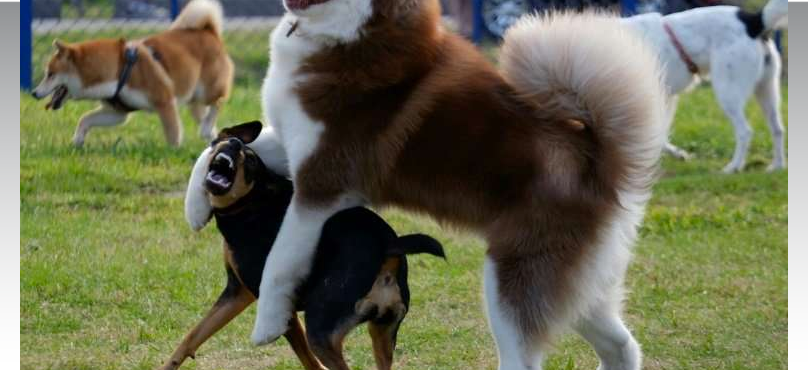
\includegraphics[width=.95\linewidth]{img/fig1.png} \quad
	\caption
	{
	Schematic describing the basic configurations
	}\label{fig:ch03f1}
\end{figure}

\paragraph{paragraph:}
\lipsum[1]
%*******************************************************

\subsection{subsection223}\label{subsection223}
\lipsum[1-3]
\paragraph{paragraph:}
\lipsum[1]
%*******************************************************

\subsection{subsection224}\label{subsection224}
\lipsum[1]
\paragraph{paragraph:}
\lipsum[1-3]
%*******************************************************

\subsubsection{subsection225}\label{subsection225}
\lipsum[1]
%*******************************************************

\subsection{subsection226}\label{subsection226}
\lipsum[1-2]
\paragraph{paragraph:}
\lipsum[1]
\paragraph{paragraph: }
\lipsum[1]
%*******************************************************
\chapter*{Conclusions }\label{conclusions}
\addcontentsline{toc}{chapter}{Conclusions}

\lipsum[1]

The work described in chapter \nameref{section11} (\autoref{subsection225})
aimed for the preparation\cite{T40} of
state of the art \ce{WS2} in \acs{SC} with help of \acs{AFM}.


\lipsum[2-9]

% now enable appendix numbering format and include any appendices
% \appendix
% \include{chapters/appendix1}
% \include{chapters/appendix2}
%*******************************************************
% Bliography
%*******************************************************
\printbibheading[heading=bibintoc]
\printbibliography[heading=subbibliography,type=article,title={Articles}]
\printbibliography[heading=subbibliography,type=book,title={Monographs \& Textbooks}]
%*******************************************************
% Other Stuff in the Back
%*******************************************************
\cleardoublepage%*******************************************************
% Colophon
%*******************************************************

\pagestyle{empty}

\hfill

\vfill


\pdfbookmark[0]{Colophon}{colophon}
\section*{Colophon}
This document was typeset using \LaTeX
The style was created by Bartlomiej Tywoniuk and is freely available here: \\
\url{https://github.com/btywoniuk/TCD_latex}

Thank you very much for your feedback and contribution.

\bigskip

\noindent


% ******************************************************
% Game Over: Restore, Restart, or Quit?
%*******************************************************
\end{document}

